% !TEX program = xelatex
\documentclass[12pt,a4paper,fontset=fandol]{ctexart}
\usepackage[left=22mm,right=22mm,top=22mm,bottom=22mm]{geometry}
\usepackage{amsmath,amssymb,bm,mathtools}
\usepackage{graphicx,xcolor,booktabs,longtable,array,calc}
\usepackage{tikz}
\usetikzlibrary{arrows.meta,calc,decorations.pathmorphing}
\usepackage{setspace,enumitem,fancyhdr}
\usepackage[unicode,hidelinks]{hyperref}
\setstretch{1.24}
\setlength{\parindent}{2em}
\setlength{\parskip}{.35em}
\setlength{\emergencystretch}{2em}
\setlist{nosep,leftmargin=2em}
\setcounter{secnumdepth}{-1}
\ctexset{section={format=\Large\bfseries,beforeskip=1em,afterskip=.7em},
subsection={format=\large\bfseries,beforeskip=.8em,afterskip=.4em},
subsubsection={format=\normalsize\bfseries,beforeskip=.7em,afterskip=.3em}}
\allowdisplaybreaks[2]
\tikzset{arr/.style={-{Stealth[length=2mm]},semithick},
dot/.style={circle,fill,inner sep=1.5pt}}
\providecommand{\tightlist}{\setlength{\itemsep}{0pt}\setlength{\parskip}{0pt}}
\providecommand{\pandocbounded}[1]{#1}
\newsavebox{\diagrambox}
\pagestyle{fancy}
\fancyhf{}
\renewcommand{\headrulewidth}{0pt}
\fancyfoot[C]{\small \thepage}
\setlength{\headheight}{16pt}
\begin{document}
\begin{titlepage}
\thispagestyle{empty}
\vspace*{27mm}
\begin{center}
{\LARGE\bfseries 第39届全国中学生物理竞赛\par}
\vspace{8mm}
{\LARGE\bfseries 复赛理论试题\par}
\vspace{17mm}
{\Large 试题版\par}
\end{center}
\vfill
\end{titlepage}
\setcounter{page}{1}
本卷共7题，总分320分。考试时间：9:00-12:00。所有需要评阅的解答均须写在答题纸上。

\section{第 1
题　迈克尔逊干涉与液体折射率（40分）}\label{ux7b2c-1-ux9898-ux8fc8ux514bux5c14ux900aux5e72ux6d89ux4e0eux6db2ux4f53ux6298ux5c04ux738740ux5206}

迈克尔逊干涉仪的入射单色激光经过半反半透镜，分成沿两个互相垂直的臂传播的光束。分光片与入射光轴成\(45^\circ\)。臂端反射镜均垂直于相应臂，并能沿臂平移。返回的两束光在空间重叠而发生干涉。照明光为发散光时，观察到同心圆环。

分光片是在平整石英基板上蒸镀薄金属膜制成。两束参与叠加的光均在分光片反射一次，但分别在石英---金属、空气---金属界面反射；两种反射的相位突变之差记为\(\Delta\varphi\)。

\begin{center}
\begin{minipage}{\linewidth}
\centering\begingroup\sbox{\diagrambox}{\small
\begin{tikzpicture}[scale=1]
\draw[arr,blue] (-3,0)--(-.15,0); \node[above] at (-2.3,0) {发散激光};
\draw[very thick] (-.55,-.55)--(.55,.55); \node[below right] at (.6,-.5) {分光片};
\draw[arr,blue] (0,.1)--(0,2.4); \draw[arr,blue] (.12,2.4)--(.12,.2);
\draw[very thick] (-.7,2.5)--(.7,2.5); \node[above] at (0,2.6) {$M_1$};
\draw[arr,red] (.15,0)--(3,0); \draw[arr,red] (3,-.12)--(.2,-.12);
\draw[very thick] (3.1,-.7)--(3.1,.7); \node[right] at (3.2,.5) {$M_2$};
\draw[arr] (0,-.2)--(0,-2); \node[below] at (0,-2) {观察方向};
\draw[<->] (3.8,-.45)--(4.6,-.45); \node at (4.2,-.9) {平移};
\end{tikzpicture}
}
\ifdim\wd\diagrambox>.88\linewidth
\sbox{\diagrambox}{\resizebox{.88\linewidth}{!}{\usebox{\diagrambox}}}\fi
\ifdim\ht\diagrambox>.20\textheight
\resizebox{!}{.20\textheight}{\usebox{\diagrambox}}
\else\usebox{\diagrambox}\fi
\par\smallskip{\small 图1a　两臂光路及反射镜的平移方向\par}\endgroup\end{minipage}\end{center}

开始时，干涉场中心为亮斑，最外侧为亮圆环，计及中心共20个亮条纹。缓慢平移一个臂的反射镜，发现圆环越来越稀疏；中心明暗变化23个周期，视场最外侧变化20个周期。条纹计数均视为精确值，两臂长度在厘米量级。

（1）求\(\Delta\varphi\)。

（2）移动后可观察到多少个亮条纹，计及中心亮斑？

（3）将扁平石英空槽插入一臂，使槽表面垂直于臂。把槽倾斜\(\theta=5.00^\circ\)时，中心变化10个周期。注入待测液体后，再将槽恢复到垂直于臂，中心变化17个周期。光波长\(\lambda=633\,\mathrm{nm}\)，槽内壁间距\(t=2.00\,\mathrm{mm}\)，空气折射率1.00。求液体折射率。

\begin{center}
\begin{minipage}{\linewidth}
\centering\begingroup\sbox{\diagrambox}{\small
\begin{tikzpicture}[scale=1]
\draw[fill=blue!6] (0,0) rectangle(5,-1.7);
\coordinate (O) at (1,0); \coordinate (B) at (2.15,-1.7);
\draw[arr] (-.4,1.4)--(O); \draw[arr] (O)--(B); \draw[arr] (B)--(3.55,-3.1);
\draw[dashed] (1,1.35)--(1,-2.4); \draw[dashed] (2.15,-1.2)--(2.15,-2.8);
\draw (1,.7) arc(90:135:.7); \node at (.65,.85) {$\theta$};
\node at (1.28,-.65) {$i$}; \node at (4,-.8) {$n$};
\draw[<->] (5.35,0)--(5.35,-1.7) node[midway,right] {$t$};
\node at (2.4,1.85) {平行液层：$\sin\theta=n\sin i$};
\node at (2.4,-3.55) {须比较同一出射波前，不能只比较斜程};
\end{tikzpicture}
}
\ifdim\wd\diagrambox>.88\linewidth
\sbox{\diagrambox}{\resizebox{.88\linewidth}{!}{\usebox{\diagrambox}}}\fi
\ifdim\ht\diagrambox>.20\textheight
\resizebox{!}{.20\textheight}{\usebox{\diagrambox}}
\else\usebox{\diagrambox}\fi
\par\smallskip{\small 图1b　倾斜平行液层的折射几何\par}\endgroup\end{minipage}\end{center}

\clearpage

\section{第 2
题　通电弹簧的平衡与稳定性（40分）}\label{ux7b2c-2-ux9898-ux901aux7535ux5f39ux7c27ux7684ux5e73ux8861ux4e0eux7a33ux5b9aux602740ux5206}

长直弹簧由涂绝缘漆的磷铜细丝绕制\(N\)匝，可视为半径\(r\)的长直螺线管。原长\(l_0\gg r\)，劲度系数\(k\)。形变时螺线管始终均匀密绕，半径变化可忽略。不计边缘效应、漏磁和重力，真空磁导率\(\mu_0\)。

（1）恒流源通过柔软导线给螺线管通以不变电流\(I_0\)，用外力使其无形变，随后缓慢撤除外力。新平衡长度\(l_p\)，弹簧仍可压缩或拉伸。

（i）导出可求\(l_p\)的代数方程，不必求解；求平衡附近小形变的等效弹性系数\(k_{\rm eff}\)，可含\(l_p\)。

（ii）求能实现平衡状态的\(I_0\)范围，不得含\(l_p\)。

（2）改用零电阻柔软导线把弹簧两端连接为闭合回路，并假设弹簧电阻也为零。初始电流\(I'_0\)，仍先用外力保持原长，再缓慢撤除。求新的平衡长度\(l'_p\)及等效弹性系数\(k'_{\rm eff}\)。

\begin{center}
\begin{minipage}{\linewidth}
\centering\begingroup\sbox{\diagrambox}{\small
\begin{tikzpicture}[scale=.9]
\draw[decorate,decoration={coil,aspect=.45,segment length=5mm,amplitude=4mm},thick] (0,0)--(6,0);
\draw[arr] (.2,-1)--(-1,-1) node[left] {$F_{\rm hold}$};
\draw[arr] (5.8,-1)--(7,-1) node[right] {$F_{\rm hold}$};
\draw[<->] (0,.9)--(6,.9) node[midway,above] {$l$};
\draw (0,0)--(0,-2)--(6,-2)--(6,0);
\draw[fill=white] (2.5,-2.4) rectangle(3.5,-1.6);
\node at (3,-2) {电路}; \node at (3,-2.95) {恒流源或理想闭合回路};
\node at (3,1.65) {$\mathcal L(l)=\mu_0\pi N^2r^2/l$};
\end{tikzpicture}
}
\ifdim\wd\diagrambox>.88\linewidth
\sbox{\diagrambox}{\resizebox{.88\linewidth}{!}{\usebox{\diagrambox}}}\fi
\ifdim\ht\diagrambox>.20\textheight
\resizebox{!}{.20\textheight}{\usebox{\diagrambox}}
\else\usebox{\diagrambox}\fi
\par\smallskip{\small 图2a　弹簧、保持力和两种供电约束\par}\endgroup\end{minipage}\end{center}

\clearpage

\section{第 3
题　实心球在粗糙斜面上的多次弹性碰撞（40分）}\label{ux7b2c-3-ux9898-ux5b9eux5fc3ux7403ux5728ux7c97ux7cd9ux659cux9762ux4e0aux7684ux591aux6b21ux5f39ux6027ux78b0ux649e40ux5206}

质量\(m\)、半径\(R\)的均匀实心球从倾角\(\theta\)的无限长固定斜面上发射，球心初速度垂直于斜面，大小\(V\)，初始自转角速度为零。建立斜面坐标系：\(x\)沿斜面向下，\(y\)垂直于斜面向上。

球与斜面碰撞是弹性的，碰撞时间极短，碰撞前后法向速度大小不变。斜面足够粗糙，碰撞时摩擦足够大、接触点无相对滑动。球绕直径的转动惯量为\(I=2mR^2/5\)。

\begin{center}
\begin{minipage}{\linewidth}
\centering\begingroup\sbox{\diagrambox}{\small
\begin{tikzpicture}[scale=.9]
\draw[thick] (-.8,0)--(8,0); \draw[arr] (0,0)--(8.4,0) node[right] {$x$};
\draw[arr] (0,0)--(0,3.5) node[above] {$y$};
\draw[thick,blue,domain=0:6,samples=80] plot(\x,{1.65*sqrt(\x)-.674*\x});
\draw[arr] (0,.3)--(0,1.25) node[left] {$V$};
\draw[arr] (2.5,3.1)--(3.6,1.8) node[right] {$\boldsymbol g$};
\node at (5,3.8) {$a_x=g\sin\theta,\quad a_y=-g\cos\theta$};
\node at (4,-.7) {每次离面法向速度相同，飞行时间均为$T$};
\end{tikzpicture}
}
\ifdim\wd\diagrambox>.88\linewidth
\sbox{\diagrambox}{\resizebox{.88\linewidth}{!}{\usebox{\diagrambox}}}\fi
\ifdim\ht\diagrambox>.20\textheight
\resizebox{!}{.20\textheight}{\usebox{\diagrambox}}
\else\usebox{\diagrambox}\fi
\par\smallskip{\small 图3a　斜面坐标下的飞行段\par}\endgroup\end{minipage}\end{center}

求：（1）第一次碰撞前球心速度和自转角速度；（2）第一次碰撞后两者；（3）第\(n\)次碰撞后球心沿\(x\)方向的速度和自转角速度；（4）前\(n\)次碰撞中斜面对球施加的总冲量。

\clearpage

\section{第 4
题　随圆环转动的铰接细杆（60分）}\label{ux7b2c-4-ux9898-ux968fux5706ux73afux8f6cux52a8ux7684ux94f0ux63a5ux7ec6ux674660ux5206}

匀质刚性细杆长\(2a\)、质量\(m\)，一端小孔嵌套在半径\(R\)的水平圆环的固定点\(P\)。\(P\)随圆环绕中心竖直轴以恒定角速度\(\omega\)转动；杆同时可绕\(P\)无摩擦转动，且杆与矢径\(OP\)始终在同一竖直平面内。杆与竖直向上方向的夹角为\(\theta\)，由竖直向上转向径向外侧的方向为正，重力加速度\(g\)。

\begin{center}
\begin{minipage}{\linewidth}
\centering\begingroup\sbox{\diagrambox}{\small
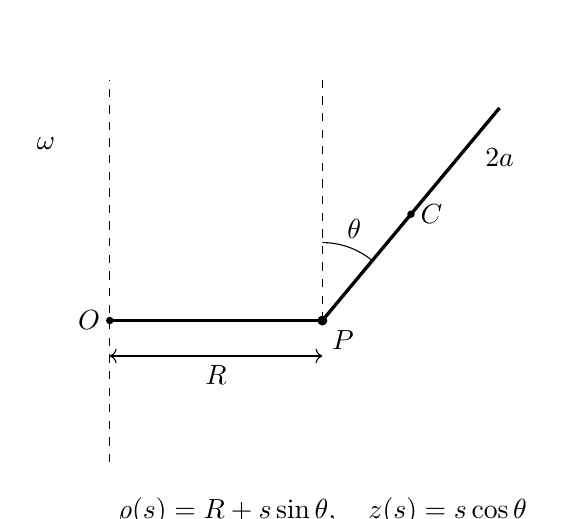
\begin{tikzpicture}[scale=.9]
\draw[dashed] (-3,-2)--(-3,3.4); \fill (-3,0) circle(1.5pt) node[left] {$O$};
\draw[thick] (-3,0)--(0,0); \fill (0,0) circle(2pt) node[below right] {$P$};
\draw[very thick] (0,0)--(2.5,3);
\draw[dashed] (0,0)--(0,3.5);
\draw (0,1.1) arc(90:50.2:1.1); \node at (.45,1.3) {$\theta$};
\fill (1.25,1.5) circle(1.5pt) node[right] {$C$};
\draw[<->] (-3,-.5)--(0,-.5) node[midway,below] {$R$};
\node at (2.5,2.3) {$2a$}; \node at (-3.9,2.5) {$\omega$};
\node at (0,-2.7) {$\varrho(s)=R+s\sin\theta,\quad z(s)=s\cos\theta$};
\end{tikzpicture}
}
\ifdim\wd\diagrambox>.88\linewidth
\sbox{\diagrambox}{\resizebox{.88\linewidth}{!}{\usebox{\diagrambox}}}\fi
\ifdim\ht\diagrambox>.20\textheight
\resizebox{!}{.20\textheight}{\usebox{\diagrambox}}
\else\usebox{\diagrambox}\fi
\par\smallskip{\small 图4a　几何、角度和质心位置\par}\endgroup\end{minipage}\end{center}

（1）将所有保守力的功与势能变化联系，分别在实验室系\(L\)和随\(OP\)转动的系\(S\)写出杆的机械能，可含\(\theta\)。

（2）在\(S\)中导出平衡位形满足的条件。

（3）用图解法分析各象限可能的平衡数目及\(a,R,\omega\)的条件。四象限依次为\([0,\pi/2)\)、\([\pi/2,\pi)\)、\([\pi,3\pi/2)\)、\([3\pi/2,2\pi)\)。

（4）在\(S\)中分象限画出对\(P\)点力矩有贡献的受力图，分布力可用力矩等效力示意，检验（3）。

（5）讨论各平衡位形的稳定性。

\clearpage

\section{第 5
题　两根弹簧的断裂先后（40分）}\label{ux7b2c-5-ux9898-ux4e24ux6839ux5f39ux7c27ux7684ux65adux88c2ux5148ux540e40ux5206}

两根相同理想轻弹簧，劲度系数\(k\)，自然长度均为零，中间连接质量\(m\)的小球。弹簧1上端固定于天花板，弹簧2在小球下方，初始下端自由，系统自然下垂且静止。任一弹簧伸到相同临界长度便断裂，该长度大于\(mg/k\)。

实验中，缓慢拉下弹簧2下端，弹簧1会先断；快速拉动时，很有可能弹簧2先断。

\begin{center}
\begin{minipage}{\linewidth}
\centering\begingroup\sbox{\diagrambox}{\small
\begin{tikzpicture}[scale=1]
\draw[thick] (-1,3)--(1,3);
\draw[decorate,decoration={coil,aspect=.4,segment length=3mm,amplitude=3mm}] (0,3)--(0,.6);
\draw[fill=gray!15] (0,.3) circle(.3); \node[right] at (.4,.3) {$m$};
\draw[decorate,decoration={coil,aspect=.4,segment length=3mm,amplitude=3mm}] (0,0)--(0,-2);
\draw[arr] (0,-2)--(0,-3.1) node[right] {$F(t)=\alpha t$};
\draw[<->] (-.8,3)--(-.8,.3) node[midway,left] {$x_1$};
\draw[<->] (.8,.3)--(.8,-2) node[midway,right] {$x_2$};
\node at (1.8,2) {弹簧1}; \node at (1.8,-1.8) {弹簧2};
\draw[arr] (3.7,1.1)--(3.7,-.25);
\node[align=center] at (3.7,-.85) {向下\\为正};
\end{tikzpicture}
}
\ifdim\wd\diagrambox>.88\linewidth
\sbox{\diagrambox}{\resizebox{.88\linewidth}{!}{\usebox{\diagrambox}}}\fi
\ifdim\ht\diagrambox>.20\textheight
\resizebox{!}{.20\textheight}{\usebox{\diagrambox}}
\else\usebox{\diagrambox}\fi
\par\smallskip{\small 图5a　上、下弹簧与力加载\par}\endgroup\end{minipage}\end{center}

（1）加载于弹簧2下端的力为\(F(t)\)，写弹簧1长度\(x_1(t)\)与小球加速度满足的方程。

（2）设\(F(t)=0\)（\(t<0\)），\(F(t)=\alpha t\)（\(t\geq0\)），\(\alpha>0\)。求\(t>0\)时两弹簧长度。

（3）设先断时刻\(t_0\)：（i）求弹簧1必然先断的\(\alpha\)范围；（ii）其他\(\alpha\)下，弹簧1先断的\(t_0\)应满足什么条件；（iii）分析弹簧2先断的可能性与\(\alpha\)关系，解释实验。

（4）给定临界长度\(L\)，写确保弹簧2先断的\(\alpha\)关系式。能否同时断？若能，写相应关系式。

\clearpage

\section{第 6
题　温差电效应的经典玩具模型（60分）}\label{ux7b2c-6-ux9898-ux6e29ux5deeux7535ux6548ux5e94ux7684ux7ecfux5178ux73a9ux5177ux6a21ux578b60ux5206}

厚度\(2L\)的金属平板占据\(-L<x<L\)，沿\(y,z\)无限延展，外部\(|x|>L\)为真空且电场为零。导电电子视为均匀正电荷背景上的经典理想气体。无温度梯度时电子数密度为\(n_0\)，正背景电荷密度为\(en_0\)。

有温度梯度时\(T(x)=T_0+\delta T(x)\)，\(n(x)=n_0+\delta n(x)\)，其中\(|\delta T|\ll T_0\)、\(|\delta n|\ll n_0\)。板内有小电场\(E_x(x)\)，表面\(x=\pm L\)内侧分别有小面电荷密度\(\sigma_\pm\)。电子质量\(m\)，电荷\(-e\)且\(e>0\)；忽略重力，玻尔兹曼常量\(k_B\)。

\begin{center}
\begin{minipage}{\linewidth}
\centering\begingroup\sbox{\diagrambox}{\small
\begin{tikzpicture}[scale=.9]
\draw[fill=blue!6] (0,-1.8) rectangle(6,1.8);
\draw[very thick] (0,-1.8)--(0,1.8); \draw[very thick] (6,-1.8)--(6,1.8);
\node[above] at (0,1.8) {$\sigma_-$}; \node[above] at (6,1.8) {$\sigma_+$};
\node at (3,.8) {$n=n_0+\delta n,\quad T=T_0+\delta T$};
\node at (3,-.1) {背景电荷密度$+en_0$};
\draw[arr] (-2,-2.5)--(8,-2.5) node[right] {$x$};
\node[below] at (0,-2.5) {$-L$}; \node[below] at (6,-2.5) {$L$};
\node at (-1.2,0) {$E=0$}; \node at (7.2,0) {$E=0$};
\node at (3,-1.1) {$E'=-e\delta n/\varepsilon_0$};
\end{tikzpicture}
}
\ifdim\wd\diagrambox>.88\linewidth
\sbox{\diagrambox}{\resizebox{.88\linewidth}{!}{\usebox{\diagrambox}}}\fi
\ifdim\ht\diagrambox>.20\textheight
\resizebox{!}{.20\textheight}{\usebox{\diagrambox}}
\else\usebox{\diagrambox}\fi
\par\smallskip{\small 图6a　金属平板、表面电荷与电场边界\par}\endgroup\end{minipage}\end{center}

（1）电子粒子流密度\(j_x\)满足斐克定律

\[
j_x=-D\frac{dn}{dx},\qquad
D=c\frac{\sqrt{T(x)}}{n(x)},
\]

\(c\)为已知常量。电阻率\(\rho\)为与\(n,T\)无关的常量。平衡时扩散电流与电场漂移电流相抵消，求\(E_x\)。

（2）用高斯定理求电场微分方程；消去电场，求\(n\)的微分方程及边界条件。真空介电常量\(\varepsilon_0\)，注意正电荷背景。

（3）只保留小量的一阶项，求\(\delta n(x)\)，可含\(\sigma_\pm\)。

（4）电子气在每处局域热平衡，且薄层电子气受电场力仍宏观力学平衡。导出\(\delta T\)的方程、线性化并求解。

（5）求

\[
S=\frac{U(L)-U(-L)}{T(L)-T(-L)}.
\]

原题附注：真实金属的温差电效应须考虑电子量子效应，本题简化经典模型不适用于真实情况。

\clearpage

\section{第 7
题　超相对论经典气体与火球膨胀（40分）}\label{ux7b2c-7-ux9898-ux8d85ux76f8ux5bf9ux8bbaux7ecfux5178ux6c14ux4f53ux4e0eux706bux7403ux81a8ux80c040ux5206}

大型强子对撞机的高能铅核---铅核碰撞，早期产物可视为高温``火球''。本题只考虑其中静止质量很小、速度接近光速的夸克，忽略其他组分。夸克视为质点，除相互碰撞的瞬间外无相互作用，碰撞中粒子数守恒，速度分布各向同性。

温度\(T\)时，动量大小区间\([p,p+dp]\)的粒子分布比率正比于

\[
e^{-E/(k_BT)}\,4\pi p^2\,dp.
\]

玻尔兹曼常量\(k_B\)、气体常量\(R\)视为已知。

（1）导出模型中压强\(P\)与平均能量密度\(u\)的关系。

（2）导出\(P\)、粒子数密度\(n\)、温度\(T\)之间的状态方程。

（3）求定体摩尔热容\(C_V\)和热容比\(\gamma=C_P/C_V\)。

（4）火球近似球形，初始半径\(3.0\times10^{-15}\,\mathrm m\)，温度\(400\,\mathrm{MeV}/k_B\)。膨胀降温至\(150\,\mathrm{MeV}/k_B\)时，夸克开始束缚为质子和中子。按准静态绝热过程近似，求刚开始形成核子时的火球半径。

\end{document}
